\documentclass[12pt,titlepage]{article}
\usepackage[dvipsnames,rgb,dvips,table]{xcolor}
\usepackage{graphicx}
\usepackage[font=small,labelfont=bf]{caption}
\graphicspath{{../Figures/}}
\usepackage{psfrag}
\usepackage{dcolumn}
\usepackage{bm}
\usepackage{amsmath}
\usepackage{amssymb}
\usepackage[rflt]{floatflt}
\usepackage{latexsym}
%\usepackage{float}
\usepackage{bm}
\usepackage{subcaption}
\usepackage{booktabs}
\usepackage{floatrow}
\floatsetup[table]{font=footnotesize}
\usepackage[hidelinks]{hyperref}
\usepackage{array}
\usepackage{ragged2e}
\newcolumntype{P}[1]{>{\RaggedRight\hspace{0pt}}p{#1}}
\usepackage{color}
\usepackage[bottom]{footmisc}

\usepackage[left=20mm,right=20mm,top=25mm,bottom=20mm]{geometry}


\pagestyle{myheadings}
\markright{{\small Jacopo Credi \hfill (910216-T396) \,}}
\DeclareMathOperator\erf{erf}
\author{Jacopo Credi \\(910216-T396) \\ \vspace*{2cm} }
\title{{\Large \textsc{Chalmers University of Technology}} \\ \bigskip FFR135 - Artificial Neural Networks\\ \bigskip Examples sheet 4 \\ \vspace*{2cm}}

\usepackage{listings}
\usepackage{color} %red, green, blue, yellow, cyan, magenta, black, white
\definecolor{mygreen}{RGB}{28,172,0} % color values Red, Green, Blue
\definecolor{mylilas}{RGB}{170,55,241}
% Settings for writing Matlab code
\lstset{language=Matlab,%
	basicstyle=\small\ttfamily,
    %basicstyle=\color{red},
    breaklines=true,%
    morekeywords={matlab2tikz},
    keywordstyle=\color{blue},%
    morekeywords=[2]{1}, keywordstyle=[2]{\color{black}},
    identifierstyle=\color{black},%
    stringstyle=\color{mylilas},
    commentstyle=\color{mygreen},%
    showstringspaces=false,%without this there will be a symbol in the places where there is a space
    numbers=left,%
    numberstyle={\tiny \color{black}},% size of the numbers
    numbersep=9pt, % this defines how far the numbers are from the text
    %emph=[1]{for,end,break},emphstyle=[1]\color{red}, %some words to emphasise
    frame=single,                   % adds a frame around the code
  	rulecolor=\color{black},
    %emph=[2]{word1,word2}, emphstyle=[2]{style},    
}


\setlength{\parskip}{3pt}

\begin{document}
\parindent=0cm
\maketitle

\subsection*{Task 1a}

\begin{figure}[htbp]
\centering
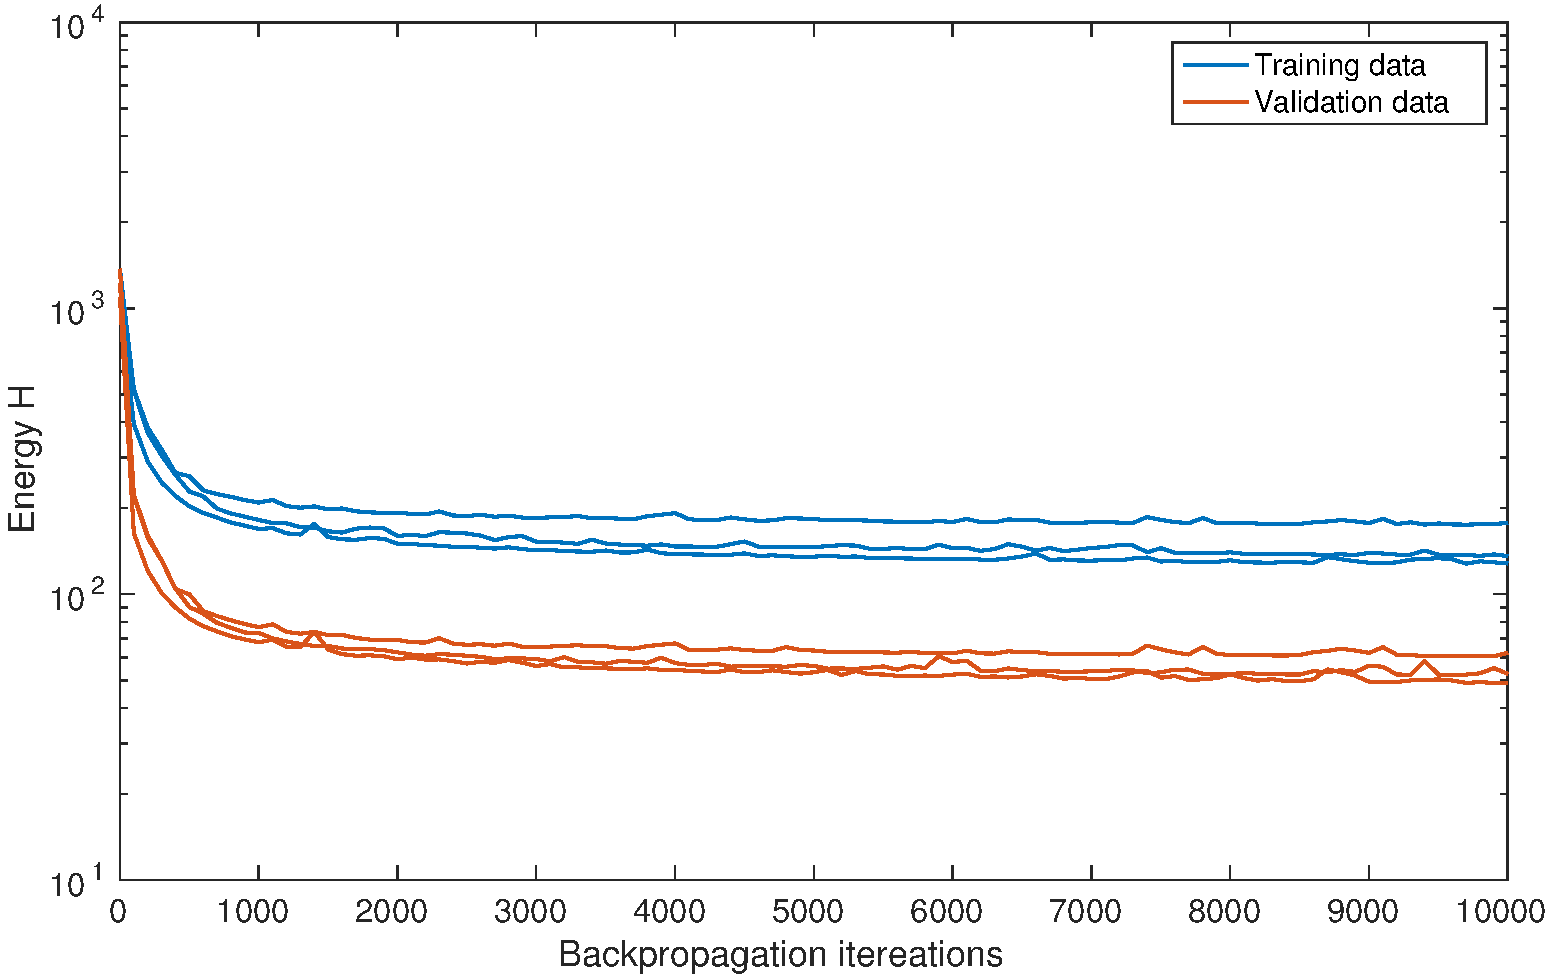
\includegraphics[width=0.75\textwidth]{1a_energy.pdf}
\caption{Energy (in log scale) vs iterations of backpropagation algorithm, for $N_G = 5$ Gaussian nodes. Training data in blue, validation data in red. For clarity, only three runs out of 20 are shown, each with only one point every 100 iterations. Parameters in the competitive learning phase: $10^5$ iterations, learning rate $\eta_c = 0.02$, neighbourhood function width $\sigma = 0.1$. Parameters in the backpropagation phase: $10^4$~iterations, learning rate $\eta_b = 0.1$, activation function $g(b) = \tanh(\beta b)$, with $\beta = 0.5$.}
\label{1a_energy}
\end{figure}

The provided data were classified using a neural network which combines unsupervised (competitive learning) and supervised learning (simple perceptron).
For the competitive learning part, $N_G = 5$ Gaussian nodes were used. Given an input vector\footnote{In this case, the data need not be normalised because we are not going to pass them (directly) through a sigmoid function, and there is no risk of zero derivative as in the perceptron case.} $\bm{x}^{\mu}$, the winning neuron (denoted by $i_0$) is the unit whose activation function is maximum: $g_{i_0}(\bm{x}^{\mu}) \geq g_{i}(\bm{x}^{\mu})$ for all $i = 1,\ldots,N_G$. After determining the winning unit, all weights are updated, according to the following learning rule:
\[
\delta \bm{w}_i \ = \ \eta \ \Lambda(i,i_0) \ (\bm{x}^{\mu}-\bm{w}_i) \ ,
\]
where the neighbouring function $\Lambda(i,i_0)$ was taken to be $\Lambda(i,i_0) = \exp{[-||i-i_0||^2/(2\sigma^2)]}$. Then, the Gaussian nodes are used as input units of a simple perceptron, trained with backpropagation. In order to do this, the data were randomly divided in two parts: one for training (70\%) and
the other for validation (the remaining 30\%).

Figure~\ref{1a_energy} shows the energy change as the backpropagation training is carried out. The energy quickly drops by a factor of $\sim8$ in the first 2000 iterations, but then does not decrease further. The average final energy values, with parameters in figure caption and $N_G = 5$ Gaussian nodes, were
\[
H^{(\textup{training})} = (14 \pm 2)\cdot 10^1, \qquad \mbox{and} \qquad H^{(\textup{validation})} = (6.0 \pm 1.1)\cdot 10^1
\]
Values are averages over 20 runs, with standard deviation. The ratio of the values reflect the size of the two datasets, as energy is extensive. We will later see (\textbf{1b}) that such values correspond to a rather poor classification performance.

\clearpage
\subsection*{Task 1b}

\begin{figure}[htbp]
\centering
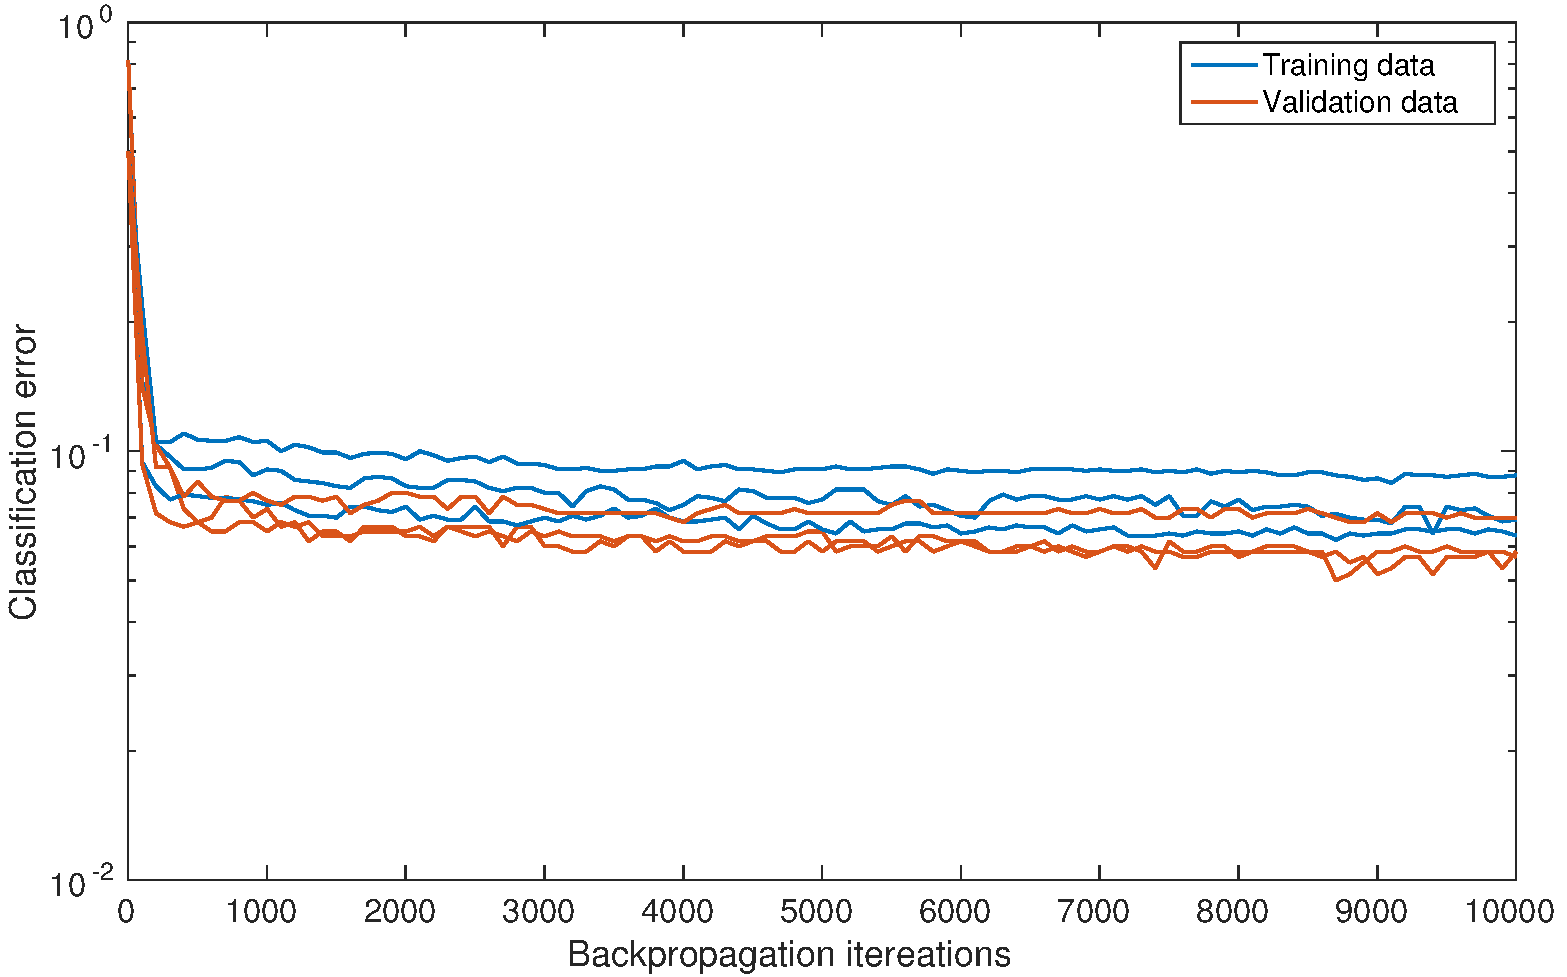
\includegraphics[width=0.8\textwidth]{1b_error.pdf}
\caption{Classification error vs iterations of backpropagation algorithm, for $N_G = 5$ Gaussian nodes. Training data in blue, validation data in red. For clarity, only three runs out of 20 are shown, each with only one point every 100 iterations. Parameters in the competitive learning phase: $10^5$ iterations, learning rate $\eta_c = 0.02$, neighbourhood function width $\sigma = 0.1$. Parameters in the backpropagation phase: $10^4$~iterations, learning rate $\eta_b = 0.1$, activation function $g(b) = \tanh(\beta b)$, with $\beta = 0.5$.}
\label{1b_error}
\end{figure}

The classification error can be computed as usual:
\[
C_V = \dfrac{1}{2 N_p} \sum_{\mu = 1}^{p} \mid \zeta^{(\mu)}-\mbox{sgn}(O^{(\mu)})\mid \ ,
\]
where $p$ is the number of data points (in this case, $p^{(\textup{training})} = 1400$ and $p^{(\textup{validation})} = 600$).

Using the same parameters as in \textbf{1a}, the classification error was computed every 100 backpropagation iterations, obtaining the plots in Fig.~\ref{1b_error} (only 3 runs out of 20 are shown, for clarity).

The final classification errors for the training and validation data sets, with parameters in figure caption and $N_G = 5$ Gaussian nodes, were
\[
C_V^{(\textup{training})} = 0.069 \pm 0.010 , \qquad \mbox{and} \qquad C_V^{(\textup{validation})} = 0.070 \pm 0.014 \ .
\]
Above values are averages over 20 runs, with standard deviation.

Although the training process can be considered complete (since both the energy and the error have reached their equilibrium value), the network ``only'' classifies 93\% of the input points correctly. We will later see that the number of Gaussian nodes has a huge impact of the classification performance.

  
\clearpage
\subsection*{Task 1c}

\begin{figure}[htbp]
\centering
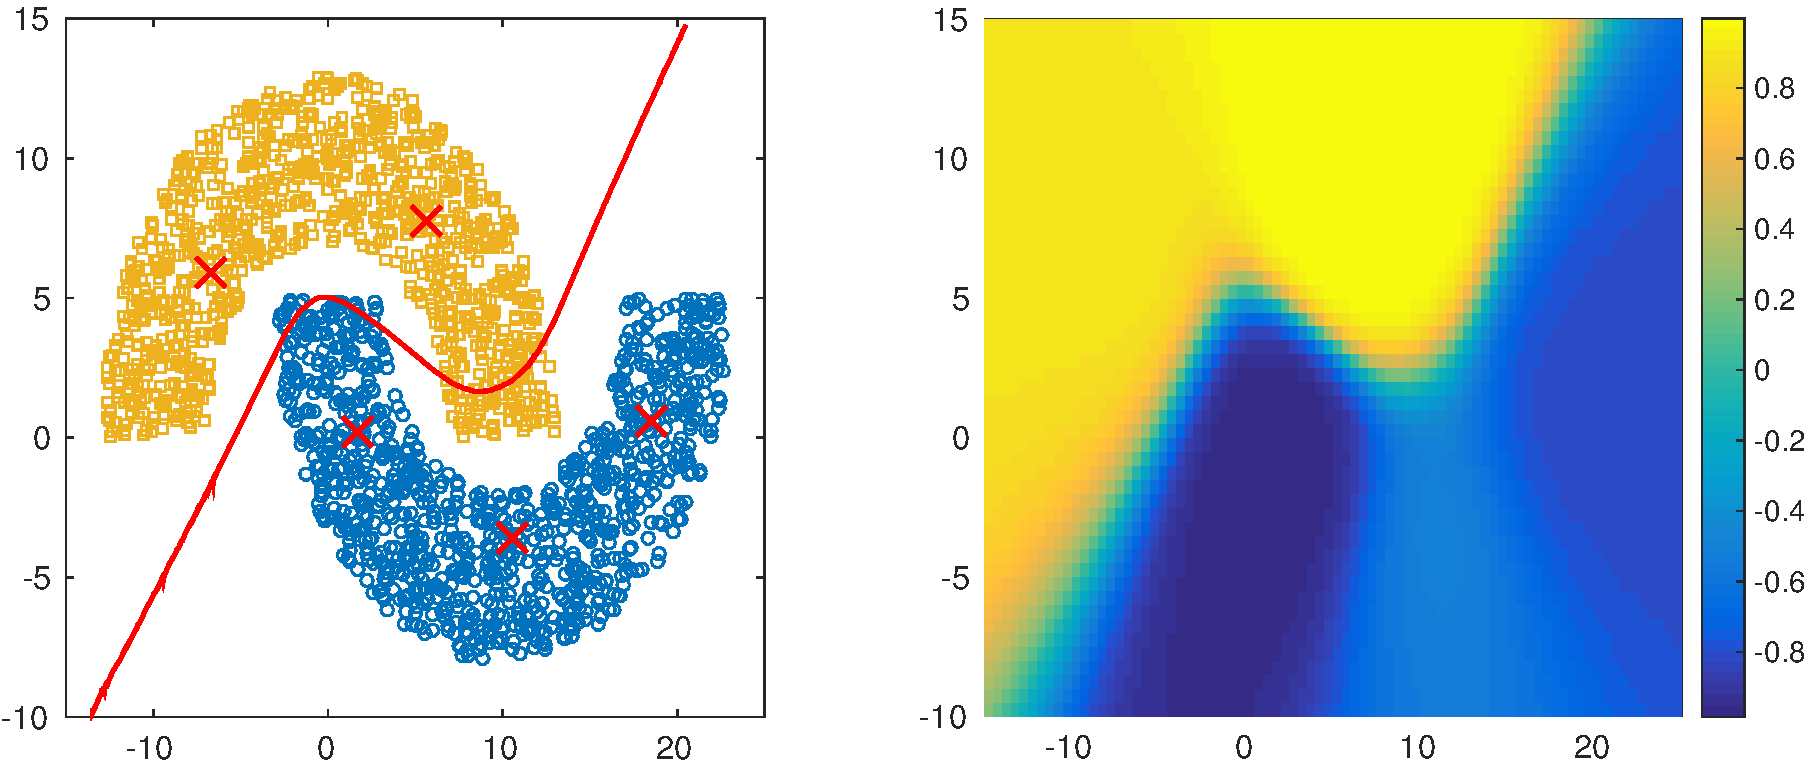
\includegraphics[width=\textwidth]{1c_boundary.pdf}
\caption{Left panel: data points, plotted in different colours and with different symbols according to the sign of the corresponding class, weight vectors as red crosses, and decision boundary as red line. Right panel: pseudo-colour map representation of the network output for a grid of equally spaced points covering the same portion of the input space. Same parameters as in \textbf{1a} and \textbf{1b}, 5 Gaussian nodes.}
\label{fig:1c_boundary}
\end{figure}

From the runs in \textbf{1a} and \textbf{1b}, the one with the best performance was chosen, i.e. the one yielding the lowest validation error (which turned out to also correspond to the lowest training error).
Then, a large number ($10^5$) of random data points were generated and fed into the neural network. For each such point, if the output was in interval $[-0.01, 0.01]$, then the point was saved, otherwise it was discarded. The set of points obtained in this way was then sorted with respect to the x-coordinate, and then plotted, to produce the red line in the left panel of Fig.~\ref{fig:1c_boundary}. In the same panel, the original data points are also plotted (in different colour, according to the corresponding class) and the Gaussian nodes weight vectors are shown as red crosses. 

We can see that the weights correctly match the data distribution, but the decision boundary is not very precise and it incorrectly classifies a bunch of data points in both clusters. It can therefore be inferred that the number of Gaussian nodes is insufficient to fully capture the distribution of the data and classify them correctly.

The pseudo-colour map in the right panel of Fig.~\ref{fig:1c_boundary}, instead, was obtained by generating a grid of equally spaced points in the input plane, passing these points through the network and colouring each point according to the network output (see colorbar).

\clearpage
\subsection*{Task 2a}

\begin{figure}[htbp]
\centering
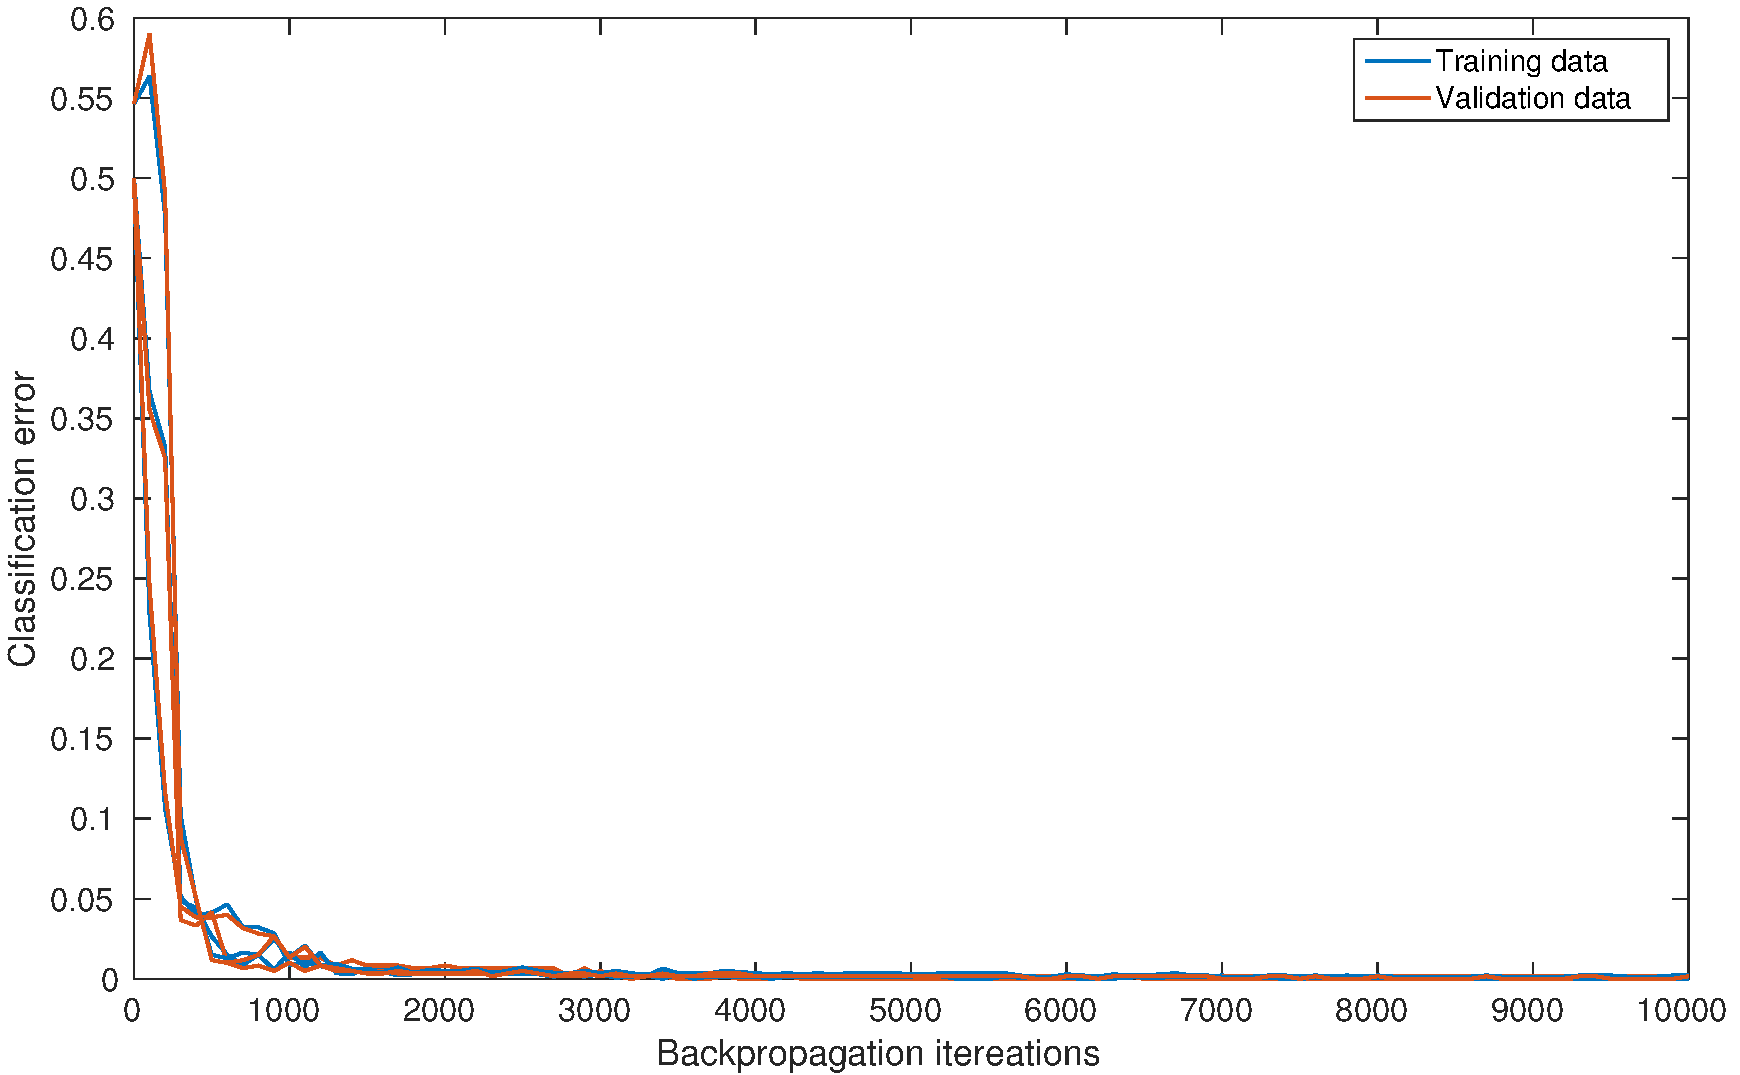
\includegraphics[width=0.8\textwidth]{2a_error.pdf}
\caption{Classification error vs iterations of backpropagation algorithm, for $N_G = 20$ Gaussian nodes. Training data in blue, validation data in red. For clarity, only three runs out of 20 are shown, each with only one point every 100 iterations. Parameters in the competitive learning phase: $10^5$ iterations, learning rate $\eta_c = 0.02$, neighbourhood function width $\sigma = 0.1$. Parameters in the backpropagation phase: $10^4$~iterations, learning rate $\eta_b = 0.1$, activation function $g(b) = \tanh(\beta b)$, with $\beta = 0.5$.}
\label{2a_error}
\end{figure}

The network architecture was then modified, increasing the number of Gaussian nodes to 20 units. As shown in Fig.~\ref{2a_error}, this led to significantly smaller classification errors, or in other terms, to a better classification performance.

The final classification errors for the training and validation data sets, with parameters in figure caption and $N_G = 20$ Gaussian nodes, were in fact
\[
C_V^{(\textup{training})} = 0.001 \pm 0.001 , \qquad \mbox{and} \qquad C_V^{(\textup{validation})} = 0.001 \pm 0.002 \ .
\]
Above values are averages over 20 runs, with standard deviation. Indeed, values are statistically compatible with zero. The network is correctly classifying input data 99.9\% of the time.


\clearpage
\subsection*{Task 2b}

\begin{figure}[htbp]
\centering
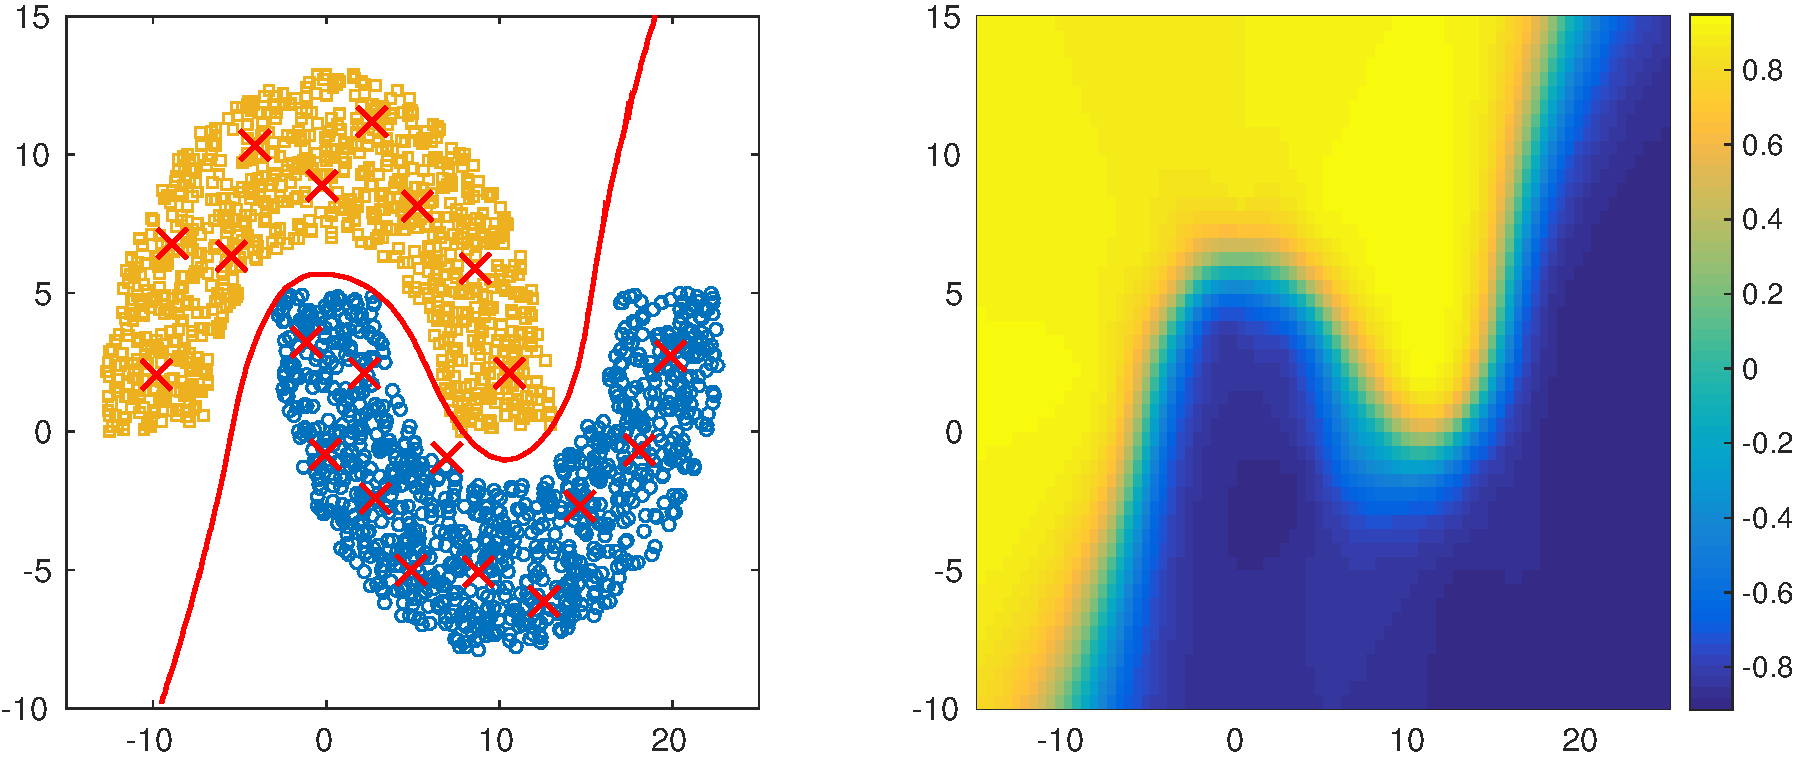
\includegraphics[width=\textwidth]{2b_boundary.pdf}
\caption{Left panel: data points, plotted in different colours and with different symbols according to the sign of the corresponding class, weight vectors as red crosses, and decision boundary as red line. Right panel: pseudo-colour map representation of the network output for a grid of equally spaced points covering the same portion of the input space. Same parameters as in \textbf{2a}, 20 Gaussian nodes.}
\label{fig:2b_boundary}
\end{figure}

From the runs in \textbf{2a}, the one with the best performance was chosen, i.e. the one yielding the lowest validation error (which again turned out to also correspond to the lowest training error).
Then, a large number ($10^5$) of random data points were generated and fed into the neural network. For each such point, if the output was in interval $[-0.01, 0.01]$, then the point was saved, otherwise it was discarded. The set of points obtained in this way was then sorted with respect to the x-coordinate, and then plotted, to produce the red line in the left panel of Fig.~\ref{fig:2b_boundary}. In the same panel, the original data points are also plotted (in different colour, according to the corresponding class) and the Gaussian nodes weight vectors are shown as red crosses. 

Again, the weights correctly match the data distribution, spreading roughly uniformly in the space covered by the two data clusters. Compared to the one obtained in \textbf{1c}, the decision boundary separates the data clusters much more accurately. It can therefore be inferred that 20 Gaussian nodes are sufficient to fully capture the distribution of the data and classify them correctly.


\clearpage
\subsection*{Task 3}

\begin{figure}[htbp]
\centering
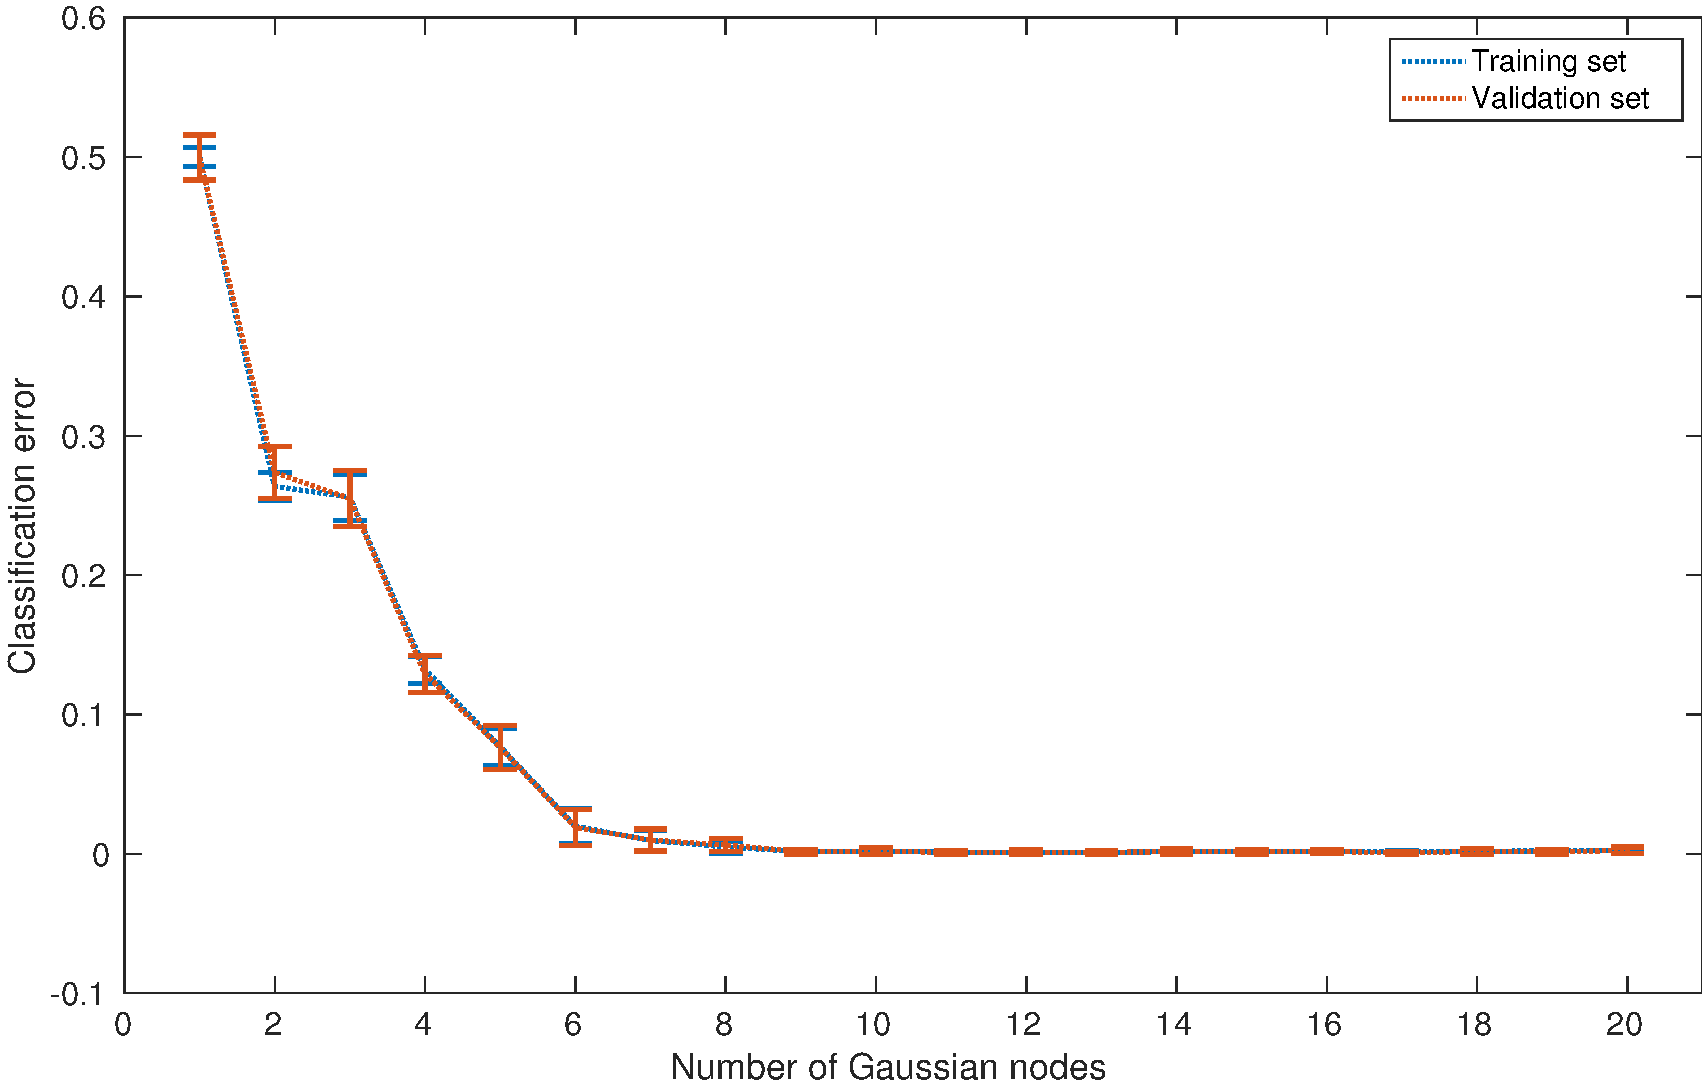
\includegraphics[width=0.8\textwidth]{3_errorVsNodes.pdf}
\caption{Classification error vs number of Gaussian nodes used for the competitive learning part. Training data in blue, validation data in red. Parameters in the competitive learning phase: $10^5$ iterations, learning rate $\eta_c = 0.02$, neighbourhood function width $\sigma = 0.1$. Parameters in the backpropagation phase: $5\cdot10^3$~iterations, learning rate $\eta_b = 0.1$, activation function $g(b) = \tanh(\beta b)$, with $\beta = 0.5$.}
\label{3_errorVsNodes}
\end{figure}

The effect of the number of Gaussian nodes on the network performance was tested by using a variable number $N_G $of nodes $N_G = 1, 2,\ldots,20$. For each value of the number of Gaussian nodes, 20 independent training runs were carried out. 

The resulting final average classification error as a function of the number of nodes is plotted in Figure~\ref{3_errorVsNodes}. Errorbars are standard deviations over the 20 runs. Errors are displayed for both the (randomly constructed) training (in blue) and validation set (in red), although points exhibit a strong overlap and are hard to distinguish.

There are two main remarks about this plot. First, with a single Gaussian node, the error is about 0.5, i.e the network is correctly classifying input points 50\% of the time, just like a random classifier would do. This is expected, since data are organised in two clusters, and this feature cannot be captured by using a single Gaussian node in the competitive unsupervised learning phase. Two Gaussian nodes, however, are still too few for a good classification, as cluster are not ``convex'' and several data points belonging to one of them are actually closer\footnote{``Closer'' here refers to both the Euclidean and the radial basis function sense.} to the ``centre'' of the \emph{other} cluster (the one that they do \emph{not} belong to).

A number of Gaussian nodes of about $9\sim 10$ appears to be sufficient to properly reconstruct the distribution of the original data and therefore train the network as a classifier, provided that the training is carried out with suitable parameters and for a sufficient number of iterations. 


\clearpage
\appendix

\section*{MATLAB code used}
\subsection*{\texttt{ClassificationProblem.m}}

\begin{lstlisting}
%% CLASSIFICATIONPROBLEM Main script for ANN - Examples sheet 4
clear; clc; close all;

%% Parameters
nRuns = 20;
nCurvesToPlot = 3;

nIterationsKohonen = 1e5;
nKohonenNodes = 20;
etaKohonen = 0.02;
sigmaNeighbourhoodFunction = 0.2;

nIterationsBackpropagation = 5e3;
nOutputNodes = 1;
etaBackpropagation = 0.1;
beta = 0.5;
nIterationsBetweenPlots = 100;

%% Load data
tmpData = importdata('../Data/data_classify.txt');
patternClasses = tmpData(:,1);
patterns = tmpData(:,2:end);
nPatterns = size(patterns, 1);

%% Loop over number of Gaussian nodes
% h = waitbar(0,'Please wait...');
% for nKohonenNodes=1:20

%% Loop over runs
for iRun = 1:nRuns
  
  fprintf('\nRUN %i:\n',iRun);
    
  % Unsupervised learning part (Kohonen)
  tic;
  kohonenWeights = CompetitiveLearning(patterns, nKohonenNodes, ...
    sigmaNeighbourhoodFunction, nIterationsKohonen, etaKohonen);
  fprintf('  - Competitive learning completed in %4.3f seconds.\n',toc);

  % Supervised learning part (backpropagation)
  tic;
  resultsStructure(iRun) = Backpropagation(patterns,patternClasses,kohonenWeights, nIterationsBackpropagation, beta, etaBackpropagation, nIterationsBetweenPlots);
  fprintf('  - Perceptron backpropagation completed in %4.3f seconds.\n',toc);  
  
end
clc;
fprintf('%i runs with %i Kohonen nodes completed.\n',nRuns,nKohonenNodes);

% Plot energy and error (3 curves)
whichOnes = randperm(nRuns,nCurvesToPlot);
[energyTrainingPlot, energyValidationPlot] = PlotEnergy(whichOnes, ...
  nIterationsBetweenPlots, nIterationsBackpropagation, resultsStructure);
[errorTrainingPlot, errorValidationPlot] = PlotError(whichOnes,...
  nIterationsBetweenPlots, nIterationsBackpropagation, resultsStructure);

% Average energy and error (with uncertainties) for training and validation
tmpEnTr = zeros(nRuns,1);
tmpEnVal = zeros(nRuns,1);
tmpErrTr = zeros(nRuns,1);
tmpErrVal = zeros(nRuns,1);
for iRun = 1:nRuns
  tmpEnTr(iRun) = resultsStructure(iRun).energyTraining(end);
  tmpEnVal(iRun) = resultsStructure(iRun).energyValidation(end);
  tmpErrTr(iRun) = resultsStructure(iRun).errorTraining(end);
  tmpErrVal(iRun) = resultsStructure(iRun).errorValidation(end);
end
avgEnergyTraining = mean(tmpEnTr);
errEnergyTraining = std(tmpEnTr);
avgEnergyValidation = mean(tmpEnVal);
errEnergyValidation = std(tmpEnVal);
avgErrorTraining = mean(tmpErrTr);
errErrorTraining = std(tmpErrTr);
avgErrorValidation = mean(tmpErrVal);
errErrorValidation = std(tmpErrVal);
[~,iBestClassifier] = min(tmpErrVal);

% errVsNodesTrainingAverage(nKohonenNodes) = avgErrorTraining;
% errVsNodesTrainingSd(nKohonenNodes) = errErrorTraining;
% errVsNodesValidationAverage(nKohonenNodes) = avgErrorValidation;
% errVsNodesValidationSd(nKohonenNodes) = errErrorValidation;

fprintf('\n  Final energy (training set): %4.3f, uncertainty: %4.3f',avgEnergyTraining,errEnergyTraining);
fprintf('\n  Final energy (validation set): %4.3f, uncertainty: %4.3f',avgEnergyValidation,errEnergyValidation);

fprintf('\n\n  Final classification error (training set): %4.3f, uncertainty: %4.3f',avgErrorTraining,errErrorTraining);
fprintf('\n  Final classification error (validation set): %4.3f, uncertainty: %4.3f\n\n',avgErrorValidation,errErrorValidation);

disp('Run script "DecisionBoundary.m" for a graphical representation of the decision boundary for the best network found.');


% waitbar(nKohonenNodes/20,h);
% end
% close(h);
\end{lstlisting}

\subsection*{CompetitiveLearning.m}
\begin{lstlisting}
function kohonenWeights = CompetitiveLearning(patterns, nKohonenNodes, ...
  sigmaNeighbourhoodFunction, nIterationsKohonen, etaKohonen)
%% CompetitiveLearning

nPatterns = size(patterns, 1);

% Initialise weights
kohonenWeights = -1 + 2*rand(nKohonenNodes,2);

% trick for speed
tmp = 1:nKohonenNodes;
A = repmat(tmp,nKohonenNodes,1)-repmat(tmp',1,nKohonenNodes);
A = triu(A) + triu(A)';
neighbourhoodMatrix = exp(-(A.^2)/(2*sigmaNeighbourhoodFunction^2));

% ===============================================================
%% Plot weights update on-the-go (cool, but not recommended for nRuns > 1)
% figure();
% hold on
% dataPlot = plot(patterns(:,1),patterns(:,2),'.','MarkerSize',12);
% weightsPlot = plot(kohonenWeights(:,1),kohonenWeights(:,2),'x');
% set(weightsPlot,'LineWidth',2,'MarkerSize',20);   
% hold off
% ===============================================================

%% Training loop
for iKohonen = 1:nIterationsKohonen
    
  iPattern = randi(nPatterns); 
  inputPattern = patterns(iPattern,:);
  
  iWinning = GetWinningNeuron(inputPattern, kohonenWeights);
  kohonenWeights = UpdateWeights(kohonenWeights, iWinning, inputPattern,...
  etaKohonen, neighbourhoodMatrix);

% ===============================================================    
%   if mod(iKohonen,1000) == 0
%     set(weightsPlot,'XData',kohonenWeights(:,1));
%     set(weightsPlot,'YData',kohonenWeights(:,2));
%     drawnow;
%   end
% ===============================================================
end

end
\end{lstlisting}

\subsection*{GetWinningNeuron.m}
\begin{lstlisting}
function iWinning = GetWinningNeuron(inputPattern, kohonenWeights)

nNodes = size(kohonenWeights,1);
activationFunction = zeros(nNodes,1);

for j = 1:nNodes
  distance = sqrt((inputPattern(1)-kohonenWeights(j,1))^2 + ...
    (inputPattern(2)-kohonenWeights(j,2))^2);
  activationFunction(j) = exp(-distance/2);
end

[~,iWinning] = max(activationFunction);

end
\end{lstlisting}



\subsection*{UpdateWeights.m}
\begin{lstlisting}
function updatedWeights = UpdateWeights(weights, iWinning, inputPattern,...
  etaKohonen, neighbourhoodMatrix)

nNodes = size(weights,1);
deltaWeights = zeros(nNodes,2);

for iNode = 1:nNodes
  tmpDiff = inputPattern-weights(iNode,:);
  deltaWeights(iNode,:) = etaKohonen*neighbourhoodMatrix(iNode,iWinning).*tmpDiff;
end

updatedWeights = weights + deltaWeights;

end
\end{lstlisting}



\subsection*{Backpropagation.m}
\begin{lstlisting}
function resultsStructure = Backpropagation(patterns, patternClasses, kohonenWeights, ...
    nIterationsBackpropagation, beta, etaBackpropagation, nIterationsBetweenPlots)
%% Backpropagation

nPatterns = size(patterns, 1);
nKohonenNodes = size(kohonenWeights,1);
nPlotPoints = 1+fix(nIterationsBackpropagation/nIterationsBetweenPlots);

% Randomly split data in training and validation sets
nTrainingData = fix(0.7*nPatterns);
trainingData = randperm(nPatterns, nTrainingData);
validationData = setdiff(1:nPatterns, trainingData);

% Initalisations
perceptronWeights = -1 + 2*rand(1,nKohonenNodes+1);
energyTraining = zeros(1, nPlotPoints);
errorTraining = zeros(1, nPlotPoints);
energyValidation = zeros(1, nPlotPoints);
errorValidation = zeros(1, nPlotPoints);
iPlot = 1;

% Compute initial energy and error
[energyTraining(iPlot), errorTraining(iPlot)] = ComputeEnergyAndError(...
patterns, patternClasses, kohonenWeights, perceptronWeights, beta);
[energyValidation(iPlot), errorValidation(iPlot)] = ComputeEnergyAndError(...
patterns, patternClasses, kohonenWeights, perceptronWeights, beta);

%======================================
%% Draw colormap on-the-go (cool, but not recommended for nRuns > 1)
%
% rangeX = [-15, 25];
% rangeY = [-10, 15];
% spacing = 0.33;
% [randomDataX,randomDataY] = meshgrid(rangeX(1):spacing:rangeX(2), rangeY(1):spacing:rangeY(2));
% nY = size(randomDataX,1);
% nX = size(randomDataX,2);
% randomDataZ = zeros(size(randomDataX));
% % Pass through classifier
% for iY = 1:nY
%   for iX = 1:nX
%     inputPattern = [randomDataX(iY,iX), randomDataY(iY,iX)];
%     [~, randomDataZ(iY,iX)] = RunClassifier(inputPattern, ...
%       kohonenWeights, nKohonenNodes, perceptronWeights, beta);
%   end
% end
% % Pseudocolor map
% pcolor(randomDataX,randomDataY,randomDataZ)
% shading flat
% axis square;
%======================================

for iBackpropagation = 1:nIterationsBackpropagation

  % pick pattern from training set
  iPattern = trainingData(randi(nTrainingData));
  inputPattern = patterns(iPattern,:);
  desiredOutput = patternClasses(iPattern);
  
  % run classifier
  [gaussianActivation, output] = RunClassifier(inputPattern, ...
    kohonenWeights, nKohonenNodes, perceptronWeights, beta);

  % backpropagation
  gPrime = beta*(1-output.^2); % because we're using g = tanh
  outputError = desiredOutput - output;
  deltaWeights = etaBackpropagation*outputError*gPrime*gaussianActivation';
  perceptronWeights = perceptronWeights + deltaWeights;
  
  % compute energy and classification error
  if mod(iBackpropagation,nIterationsBetweenPlots) == 0
    iPlot = iPlot + 1;
    [energyTraining(iPlot), errorTraining(iPlot)] = ComputeEnergyAndError(...
      patterns(trainingData,:), patternClasses(trainingData), ...
      kohonenWeights, perceptronWeights, beta);
    [energyValidation(iPlot), errorValidation(iPlot)] = ComputeEnergyAndError(...
      patterns(validationData,:), patternClasses(validationData), ...
      kohonenWeights, perceptronWeights, beta);
    
    %======================================
%     % Pass random data through classifier
%     for iY = 1:nY
%       for iX = 1:nX
%         inputPattern = [randomDataX(iY,iX), randomDataY(iY,iX)];
%         [~, randomDataZ(iY,iX)] = RunClassifier(inputPattern, ...
%           kohonenWeights, nKohonenNodes, perceptronWeights, beta);
%       end
%     end
%     % Pseudocolor map
%     pcolor(randomDataX,randomDataY,randomDataZ);
%     shading flat;
%     axis square;
%     pause(0.001);
    %======================================
  end
end

% Save results in a structure
resultsStructure.kohonenWeights = kohonenWeights;
resultsStructure.perceptronWeights = perceptronWeights;
resultsStructure.energyTraining = energyTraining;
resultsStructure.energyValidation = energyValidation;
resultsStructure.errorTraining = errorTraining;
resultsStructure.errorValidation = errorValidation;

end
\end{lstlisting}



\subsection*{RunClassifier.m}
\begin{lstlisting}
function [gaussianActivation, output] = RunClassifier(inputPattern, ...
  kohonenWeights, nKohonenNodes, perceptronWeights, beta)
%% RunClassifier

% run Kohonen network
gaussianActivation = zeros(nKohonenNodes+1,1);
for j = 1:nKohonenNodes
  distance = sqrt((inputPattern(1)-kohonenWeights(j,1))^2 + ...
    (inputPattern(2)-kohonenWeights(j,2))^2);
  gaussianActivation(j) = exp(-distance/2);
end
gaussianActivation = gaussianActivation./sum(gaussianActivation); % normalise
gaussianActivation(end) = -1; % dummy neuron (for threshold)

% run perceptron
output = tanh(beta*(perceptronWeights*gaussianActivation));
  
end
\end{lstlisting}



\subsection*{ComputeEnergyAndError.m}
\begin{lstlisting}
function [energy, classificationError] = ComputeEnergyAndError(patterns,...
  patternClasses, kohonenWeights, perceptronWeights, beta)
%% ComputeEnergyAndError    

nPatterns = size(patterns, 1);
nKohonenNodes = size(kohonenWeights,1);

tmpOutput = zeros(nPatterns,1);

for iPattern = 1:nPatterns
  inputPattern = patterns(iPattern,:);
  
  [~, tmpOutput(iPattern)] = RunClassifier(inputPattern, kohonenWeights, ...
    nKohonenNodes, perceptronWeights, beta);
end

% compute energy
tmpEnergy = (patternClasses - tmpOutput).^2;
energy = 0.5*sum(tmpEnergy);

% compute classification error
tmpError = abs(patternClasses - sign(tmpOutput)); 
classificationError = 0.5/nPatterns*sum(tmpError);

end
\end{lstlisting}



\subsection*{PlotEnergy.m}
\begin{lstlisting}
function [energyTrainingPlot, energyValidationPlot] = PlotEnergy(whichOnes,...
  nIterationsBetweenPlots, nIterationsBackpropagation, resultsStructure)
%% PlotEnergy

xValues = 1:nIterationsBetweenPlots:(nIterationsBackpropagation+1);
nCurvesToPlot = numel(whichOnes);

parulaColours = get(groot,'DefaultAxesColorOrder');
defaultBlue = parulaColours(1,:);
defaultRed = parulaColours(2,:);

figure('Units','normalized','OuterPosition',[0.15 0.15 0.7 0.7]);
set(gcf, 'Color','w');
hold on

for i = 1:nCurvesToPlot
    
  iPlot = whichOnes(i);
  
  % training
  energyTrainingPlot(iPlot) = semilogy(xValues,resultsStructure(iPlot).energyTraining);
  set(energyTrainingPlot(iPlot),'Color',defaultBlue,'LineWidth',1.5);
  
  % validation
  energyValidationPlot(iPlot) = semilogy(xValues,resultsStructure(iPlot).energyValidation);
  set(energyValidationPlot(iPlot),'Color',defaultRed,'LineWidth',1.5);
  
end

set(gca,'yscale','log','FontSize',16);
xlabel('Backpropagation itereations');
ylabel('Energy H');
xlim([0,nIterationsBackpropagation]);
set(0, 'DefaultAxesBox', 'on');
legend([energyTrainingPlot(iPlot), energyValidationPlot(iPlot)],'Training data','Validation data');
pbaspect([1.618 1 1])
hold off

end
\end{lstlisting}



\subsection*{PlotError.m}
\begin{lstlisting}
function [errorTrainingPlot, errorValidationPlot] = PlotError(whichOnes,...
  nIterationsBetweenPlots, nIterationsBackpropagation, resultsStructure)
%% PlotError

xValues = 1:nIterationsBetweenPlots:(nIterationsBackpropagation+1);
nCurvesToPlot = numel(whichOnes);

parulaColours = get(groot,'DefaultAxesColorOrder');
defaultBlue = parulaColours(1,:);
defaultRed = parulaColours(2,:);

figure('Units','normalized','OuterPosition',[0.15 0.15 0.7 0.7]);
set(gcf, 'Color','w');
hold on

for i = 1:nCurvesToPlot
    
  iPlot = whichOnes(i);
  
  % training
  errorTrainingPlot(iPlot) = plot(xValues,resultsStructure(iPlot).errorTraining);
  set(errorTrainingPlot(iPlot),'Color',defaultBlue,'LineWidth',1.5);
  
  % validation
  errorValidationPlot(iPlot) = plot(xValues,resultsStructure(iPlot).errorValidation);
  set(errorValidationPlot(iPlot),'Color',defaultRed,'LineWidth',1.5);
  
end

set(gca,'FontSize',16);
xlabel('Backpropagation itereations');
ylabel('Classification error');
xlim([0,nIterationsBackpropagation]);
set(0, 'DefaultAxesBox', 'on');
legend([errorTrainingPlot(iPlot), errorValidationPlot(iPlot)],'Training data','Validation data');
pbaspect([1.618 1 1])
hold off

end
\end{lstlisting}



\subsection*{DecisionBoundary.m}
\begin{lstlisting}
%% DECISIONBOUNDARY Script to draw decision boundary and colormap

nRandomData = 1e5;
rangeX = [-15, 25];
rangeY = [-10, 15];
spacing = 0.5;
beta = 0.5;
threshold = 0.01;

bestKohonenWeights = resultsStructure(iBestClassifier).kohonenWeights;
bestPerceptronWeights = resultsStructure(iBestClassifier).perceptronWeights;

%% Initialise plot
figure('Units','normalized','OuterPosition',[0.15 0.15 0.7 0.7]);
set(gcf, 'Color','w');
hold on
parulaColours = get(groot,'DefaultAxesColorOrder');
colour1 = parulaColours(1,:);
colour2 = parulaColours(3,:);

%% Generate random data (for decision boundary)
randomDataX = rangeX(1) + diff(rangeX)*rand(nRandomData,1);
randomDataY = rangeY(1) + diff(rangeY)*rand(nRandomData,1);
randomDataZ = zeros(nRandomData,1);
% Pass through classifier
for iRandomData = 1:nRandomData
    inputPattern = [randomDataX(iRandomData), randomDataY(iRandomData)];
    [~, randomDataZ(iRandomData)] = RunClassifier(inputPattern, bestKohonenWeights, ...
      nKohonenNodes, bestPerceptronWeights, beta);
end
% Generate decision boundary
decisionBoundaryX = randomDataX(abs(randomDataZ) < threshold);
decisionBoundaryY = randomDataY(abs(randomDataZ) < threshold);
[decisionBoundaryX, order] = sort(decisionBoundaryX);
decisionBoundaryY = decisionBoundaryY(order);

% Subplot 1
subplot(1,2,1);
plotCluster1 = plot(patterns(1:1000,1),patterns(1:1000,2));
set(plotCluster1,'LineStyle','none','Marker','s','MarkerSize',6,'LineWidth',1,'Color',colour2);
hold on

plotCluster2 = plot(patterns(1001:end,1),patterns(1001:end,2),'o','MarkerSize',10);
set(plotCluster2,'LineStyle','none','Marker','o','MarkerSize',6,'LineWidth',1,'Color',colour1);

plotWeights = plot(bestKohonenWeights(:,1),bestKohonenWeights(:,2),'x');
set(plotWeights,'LineWidth',2,'MarkerSize',16,'Color','r');   

plotDecisionBoundary = plot(decisionBoundaryX, decisionBoundaryY,'r','LineWidth',2);
set(gca,'FontSize',16);
axis square;
xlim([-15, 25]);
hsp1 = get(gca, 'Position');
hold off

%% Generate meshgrid (for pseudo-colour map)
[meshGridX,meshGridY] = meshgrid(rangeX(1):spacing:rangeX(2), rangeY(1):spacing:rangeY(2));
nY = size(meshGridX,1);
nX = size(meshGridX,2);
meshGridZ = zeros(size(meshGridX));
% Pass through classifier
for iY = 1:nY
  for iX = 1:nX
    inputPattern = [meshGridX(iY,iX), meshGridY(iY,iX)];
    [~, meshGridZ(iY,iX)] = RunClassifier(inputPattern, ...
      bestKohonenWeights, nKohonenNodes, bestPerceptronWeights, beta);
  end
end

% Plot pseudo-colour map
subplot(1,2,2);
pcolor(meshGridX,meshGridY,meshGridZ)
shading flat
axis square;
hsp2 = get(gca, 'Position');
colorbar;
set(gca,'FontSize',16);
set(gca, 'Position', [hsp2(1:2) hsp1(3:4)]);
\end{lstlisting}

\end{document}